\documentclass{beamer}

\usepackage{tikz}
\usetikzlibrary{quantikz2, backgrounds}
\usepackage{graphicx}

\usetikzlibrary{decorations.markings}

\title{T-State cultivation : circuit designs}
\author{Dynerowicz S.}
\date{}

% Taken from https://tex.stackexchange.com/questions/126119/tex-custom-arrow-with-oplus-symbol
\makeatletter
\pgfarrowsdeclare{oplus}{oplus}{%
  \pgfarrowsleftextend{+-.5\pgflinewidth}
  \pgfutil@tempdima=0.4pt%
  \advance\pgfutil@tempdima by.2\pgflinewidth%
  \pgfutil@tempdimb=9\pgfutil@tempdima\advance\pgfutil@tempdimb by.5\pgflinewidth
  \pgfarrowsrightextend{+\pgfutil@tempdimb}%
}{%
  \pgfutil@tempdima=0.4pt%
  \advance\pgfutil@tempdima by.2\pgflinewidth%
  \pgfsetdash{}{+0pt}%
  \pgfpathcircle{\pgfqpoint{4.5\pgfutil@tempdima}{0bp}}{4.5\pgfutil@tempdima}%
  \pgfpathmoveto{\pgfqpoint{0bp}{0bp}}%
  \pgfpathlineto{\pgfqpoint{9\pgfutil@tempdima}{0bp}}%
  \pgfpathmoveto{\pgfqpoint{4.5\pgfutil@tempdima}{4.5\pgfutil@tempdima}}%
  \pgfpathlineto{\pgfqpoint{4.5\pgfutil@tempdima}{-4.5\pgfutil@tempdima}}%
  \pgfusepathqstroke
}
\makeatother

\tikzstyle{quantumR}=[red!75!black!50]
\tikzstyle{quantumB}=[blue!75!black!50]
\tikzstyle{quantumG}=[green!75!black!50]
\tikzstyle{quantumY}=[yellow!95!black!75]

\tikzstyle{data}=[circle, fill=black, text=white]
\tikzstyle{meas}=[circle, fill=white, draw=black, ultra thick]
\tikzstyle{stabilizer}=[draw=black]

\tikzstyle{interact}=[line width=1.25pt, shorten <= 8pt, shorten >= 12pt, Circle-oplus]
\tikzstyle{partner}=[line width=1.25pt, shorten <= 8pt, shorten >= 12pt, Circle-oplus]

\tikzstyle{entanglement}=[decorate, ultra thick,
	decoration={snake, pre length=5pt, post length=5pt, amplitude=0.5mm, segment length=2.5mm}
]

\newcommand{\Op}[1]{{\bf #1}}
\newcommand{\kett}[1]{\ket{\mbox{\tt #1}}}
\newcommand{\wn}{\wireoverride{n}}

\begin{document}
	\begin{frame}
		\titlepage
	\end{frame}

	\begin{frame}
		\frametitle{Overview : current state}
		\centering
		\scalebox{0.75}{
			\begin{quantikz}[row sep={between origins, 0.75cm}]
				& \gate[7,style={rounded corners=5pt}][3cm]{\textsc{Injection}}
				& \gate[7,style={rounded corners=5pt}][3cm]{\textsc{Syndrome}}
				& \gate[7,style={rounded corners=5pt, fill=black, inner ysep=-29pt}]{\rotatebox{90}{\color{white}\scshape Post-select}}
				& \gate[7,style={rounded corners=5pt}][3cm]{\textsc{Cultivation}}
				& \\
				&&&&& \\
				&&&&& \\
				&&&&& \\
				&&&&& \\
				&&&&& \\
				&&&&&
			\end{quantikz}
		}
	\end{frame}

	\begin{frame}
		\frametitle{Final configuration for teleportation}
		\onslide<2->{
			\begin{itemize}
				\item Superdense code cycle requires $2$ ancillas per plaquette
				\begin{itemize}
					\item not measuring data qubits used to form the GHZ states
					\item balanced by having each ancilla interact with $2$ data qubits
				\end{itemize}
			\end{itemize}
		}
		\vspace{0.4cm}
		\centering
		\scalebox{0.65}{
			\begin{tikzpicture}
				% Data qubits of the Steane Code
				\coordinate (q1) at ( 2,-4);
				\coordinate (q2) at (-2,-4);
				\coordinate (q3) at ( 2,-2);
				\coordinate (q4) at ( 4,-4);
				\coordinate (q5) at ( 2, 0);
				\coordinate (q6) at (-2, 0);
				\coordinate (q7) at ( 0,-2);

				% Extra data qubits for forming GHZ states
				\coordinate (dR) at ( 4,-2);
				\coordinate (dG) at ( 0, 0);
				\coordinate (dB) at ( 0,-4);
				\coordinate (a0) at (-1,-1);
				\coordinate (a1) at ( 1,-1);
				\coordinate (a2) at (-1,-3);
				\coordinate (a3) at ( 1,-3);
				\coordinate (a4) at ( 3,-1);
				\coordinate (a5) at ( 3,-3);

				% Plaquettes of the Steane Code
				\fill[quantumR] (q5) -- (q3) -- (q1) -- (q4) -- (dR) -- cycle;
				\fill[quantumG] (q6) -- (dG) -- (q5) -- (q3) -- (q7) -- cycle;
				\fill[quantumB] (q2) -- (q7) -- (q3) -- (q1) -- (dB) -- cycle;
	
				% Plaquettes of the Surface Code
				\fill[quantumR] (2,-6) -- (4, -6) -- (4, -7) -- (2, -7);
				\fill[quantumR] (6,-6) -- (8, -6) -- (8, -7) -- (6, -7);
				\fill[quantumB] (0,-6) -- (2, -6) -- (2, -7) -- (0, -7);
				\fill[quantumB] (4,-6) -- (6, -6) -- (6, -7) -- (4, -7);
				\fill[quantumB] (6, -6) arc[start angle=180, end angle=0, radius=1.0] -- (8, -6) -- cycle;
				\fill[quantumB] (8, -6) arc[start angle= 90, end angle=0, radius=1.0] -- (8, -7) -- cycle;
	
				\fill[quantumB, opacity=0.25] (2,-4) -- (4, -4) -- (4, -6) -- (2, -6);
				\filldraw[quantumB, opacity=0.25] (-2,-4) to[bend left=30] (0,-6) to[bend left=30] (-2,-4);

				\only<2->{
					\draw[entanglement] (dG) -- (a0);
					\draw[entanglement] (dG) -- (a1);
					\draw[entanglement] (dB) -- (a2);
					\draw[entanglement] (dB) -- (a3);
					\draw[entanglement] (dR) -- (a4);
					\draw[entanglement] (dR) -- (a5);
				}

				\only<3>{
					\draw[interact] (a0) -- (q6);
					\draw[interact] (a0) -- (q7);
					\draw[interact] (a1) -- (q5);
					\draw[interact] (a1) -- (q3);
	
					\draw[interact] (a2) -- (q2);
					\draw[interact] (a2) -- (q7);
					\draw[interact] (a3) -- (q3);
					\draw[interact] (a3) -- (q1);
	
					\draw[interact] (a4) -- (q5);
					\draw[interact] (a4) -- (q3);
					\draw[interact] (a5) -- (q1);
					\draw[interact] (a5) -- (q4);
				}

				\node[data] at ( 0, 0) {\phantom{o}};
				\node[data] at ( 4,-2) {\phantom{o}};
				\node[data] at ( 0,-4) {\phantom{o}};

				\node[data] at (q1) {\large $\mathbf{1}$};
				\node[data] at (q2) {\large $\mathbf{2}$};
				\node[data] at (q3) {\large $\mathbf{3}$};
				\node[data] at (q4) {\large $\mathbf{4}$};
				\node[data] at (q5) {\large $\mathbf{5}$};
				\node[data] at (q6) {\large $\mathbf{6}$};
				\node[data] at (q7) {\large $\mathbf{7}$};	

				\foreach \x in {-1, 1, 3}{
					\foreach \y in {-1, -3}{
						\node[meas] at (\x,\y) {};
					}
				}
				\foreach \x in {-1, 3}{ \node[meas, opacity=0.25] at (\x,-5) {}; }

				\foreach \x in {0, 2, 4, 6, 8}{ \node[data] at (\x, -6) {\phantom{o}}; }
			\end{tikzpicture}
		}	
	\end{frame}

	\begin{frame}
		\frametitle{Final configuration for teleportation}
		\onslide<2>{
			\begin{itemize}
				\item Cultivation requires $6$ ancillas
				\begin{itemize}
					\item data qubit partnered with one ancilla
					\item shared for $q_{\scriptscriptstyle 1}$, $q_{\scriptscriptstyle 7}$
				\end{itemize}
			\end{itemize}
		}
		\vspace{0.4cm}
		\centering
		\scalebox{0.65}{
			\begin{tikzpicture}
				% Data qubits of the Steane Code
				\coordinate (q1) at ( 2,-4);
				\coordinate (q2) at (-2,-4);
				\coordinate (q3) at ( 2,-2);
				\coordinate (q4) at ( 4,-4);
				\coordinate (q5) at ( 2, 0);
				\coordinate (q6) at (-2, 0);
				\coordinate (q7) at ( 0,-2);

				% Extra data qubits for forming GHZ states
				\coordinate (dR) at ( 4,-2);
				\coordinate (dG) at ( 0, 0);
				\coordinate (dB) at ( 0,-4);
				\coordinate (a0) at (-1,-1);
				\coordinate (a1) at ( 1,-1);
				\coordinate (a2) at (-1,-3);
				\coordinate (a3) at ( 1,-3);
				\coordinate (a4) at ( 3,-1);
				\coordinate (a5) at ( 3,-3);

				% Plaquettes of the Steane Code
				\fill[quantumR] (q5) -- (q3) -- (q1) -- (q4) -- (dR) -- cycle;
				\fill[quantumG] (q6) -- (dG) -- (q5) -- (q3) -- (q7) -- cycle;
				\fill[quantumB] (q2) -- (q7) -- (q3) -- (q1) -- (dB) -- cycle;
	
				% Plaquettes of the Surface Code
				\fill[quantumR] (2,-6) -- (4, -6) -- (4, -7) -- (2, -7);
				\fill[quantumR] (6,-6) -- (8, -6) -- (8, -7) -- (6, -7);
				\fill[quantumB] (0,-6) -- (2, -6) -- (2, -7) -- (0, -7);
				\fill[quantumB] (4,-6) -- (6, -6) -- (6, -7) -- (4, -7);
				\fill[quantumB] (6, -6) arc[start angle=180, end angle=0, radius=1.0] -- (8, -6) -- cycle;
				\fill[quantumB] (8, -6) arc[start angle= 90, end angle=0, radius=1.0] -- (8, -7) -- cycle;
	
				\fill[quantumB, opacity=0.25] (2,-4) -- (4, -4) -- (4, -6) -- (2, -6);
				\filldraw[quantumB, opacity=0.25] (-2,-4) to[bend left=30] (0,-6) to[bend left=30] (-2,-4);

				\only<2>{
					\draw[partner] (a0) -- (q6);
					\draw[partner] (a1) -- (q5);
					\draw[partner] (a2) -- (q2);
					\draw[partner] (a3) -- (q1);
					\draw[partner] (a3) -- (q7);
					\draw[partner] (a4) -- (q3);
					\draw[partner] (a5) -- (q4);
				}

				\node[data] at ( 0, 0) {\phantom{o}};
				\node[data] at ( 4,-2) {\phantom{o}};
				\node[data] at ( 0,-4) {\phantom{o}};

				\node[data] at (q1) {\large $\mathbf{1}$};
				\node[data] at (q2) {\large $\mathbf{2}$};
				\node[data] at (q3) {\large $\mathbf{3}$};
				\node[data] at (q4) {\large $\mathbf{4}$};
				\node[data] at (q5) {\large $\mathbf{5}$};
				\node[data] at (q6) {\large $\mathbf{6}$};
				\node[data] at (q7) {\large $\mathbf{7}$};	

				\foreach \x in {-1, 1, 3}{
					\foreach \y in {-1, -3}{
						\node[meas] at (\x,\y) {};
					}
				}
				\foreach \x in {-1, 3}{ \node[meas, opacity=0.25] at (\x,-5) {}; }

				\foreach \x in {0, 2, 4, 6, 8}{ \node[data] at (\x, -6) {\phantom{o}}; }
			\end{tikzpicture}
		}
	\end{frame}

	\begin{frame}
		\frametitle{\sc Injection --- Abstract circuit}
		\begin{itemize}
			\item Preparation of a Steane Code logical T-state on $7$ qubits
			\begin{equation*}
				\ket{\Op{T}}_{\scriptscriptstyle L} ~=~ \kett{0}_{\scriptscriptstyle L} + e^{i\pi/4}\kett{1}_{\scriptscriptstyle L}	
			\end{equation*}
		\end{itemize}
		\vspace{0.5cm}
		\begin{minipage}{0.32\textwidth}
			\centering
			\scalebox{0.6}{
				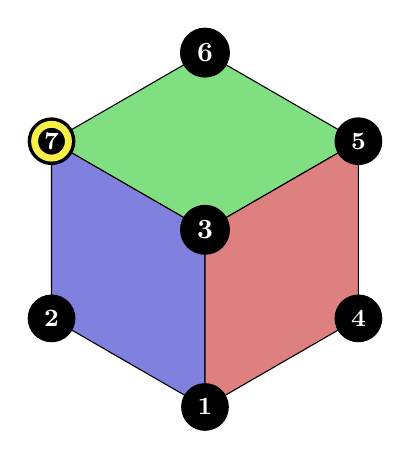
\begin{tikzpicture}
					\coordinate (O) at (0,0);
					\coordinate (A) at ( 30:2.25);
					\coordinate (B) at ( 90:2.25);
					\coordinate (C) at (150:2.25);
					\coordinate (D) at (210:2.25);
					\coordinate (E) at (270:2.25);
					\coordinate (F) at (330:2.25);
	
					\fill[quantumG, stabilizer] (O) -- (A) -- (B) -- (C) -- cycle;
					\fill[quantumB, stabilizer]  (O) -- (C) -- (D) -- (E) -- cycle;
					\fill[quantumR, stabilizer]  (O) -- (E) -- (F) -- (A) -- cycle;
	
					\node[data] at (E) {\small $\mathbf{1}$};
					\node[data] at (D) {\small $\mathbf{2}$};
					\node[data] at (O) {$\mathbf{3}$};
					\node[data] at (F) {\small $\mathbf{4}$};
					\node[data] at (A) {\small $\mathbf{5}$};
					\node[data] at (B) {$\mathbf{6}$};
					\node[data] at (C) {\small $\mathbf{7}$};
					\node[circle, draw=yellow!95!black!75, line width=2.5pt] at (C) {\phantom{.}};
				\end{tikzpicture}
			}
		\end{minipage}
		\begin{minipage}{0.62\textwidth}
			\centering
			\scalebox{0.6}{
				\begin{quantikz}[row sep=0.6cm]
					\lstick{$q_{\scriptscriptstyle 1}$}\wireoverride{n} & \midstick{$\kett{+}$~}\wireoverride{n}
					& \ctrl{1} && \ctrl{3}  && \slice{} &&&&&&
					\rstick[7]{~~$\ket{\Op{T}}_{\scriptscriptstyle L}$}
					\\
					\lstick{$q_{\scriptscriptstyle 2}$}\wireoverride{n} & \midstick{$\kett{0}$~}\wireoverride{n}
					& \targ{}  & \targ{}   &\phantom{i}& \targ{}   &
					&          & \ctrl{5}  && \ctrl{5}  &&
					\\
					\lstick{$q_{\scriptscriptstyle 3}$}\wireoverride{n} & \midstick{$\kett{+}$~}\wireoverride{n}
					& \ctrl{1} & \ctrl{-1} &\phantom{i}&\phantom{i}& \ctrl{3} &&\phantom{i}&&\phantom{i}&&
					\\
					\lstick{$q_{\scriptscriptstyle 4}$}\wireoverride{n} & \midstick{$\kett{0}$~}\wireoverride{n}
					& \targ{}  & \targ{} & \targ{}   &\phantom{i}&\phantom{i}
					&&\phantom{i}&&\phantom{i}&&
					\\
					\lstick{$q_{\scriptscriptstyle 5}$}\wireoverride{n} & \midstick{$\kett{+}$~}\wireoverride{n}
					& \ctrl{1} & \ctrl{-1} &&\phantom{i}&\phantom{i}&&\phantom{i}&&\phantom{i}&&
					\\
					\lstick{$q_{\scriptscriptstyle 6}$}\wireoverride{n} & \midstick{$\kett{0}$~}\wireoverride{n}
					& \targ{} & \targ{} &&\phantom{i}& \targ{} & \ctrl{1} &\phantom{i}&&\phantom{i}& \ctrl{1} &
					\\[-0.2cm]
					\lstick{$q_{\scriptscriptstyle 7}$}\wireoverride{n} & \midstick{$\kett{+}$~}\wireoverride{n}
					&& \ctrl{-1} && \ctrl{-5} && \targ{} & \targ{} & \gate[style={fill=yellow!95!black!75}]{\Op{T}^{\dagger}} & \targ{} & \targ{} &
				\end{quantikz}
			}
		\end{minipage}
	\end{frame}

%	\begin{frame}
%		\frametitle{\textsc{Injection} --- Actual circuit}
%		\begin{itemize}
%			\item Preparation of $\ket{\Op{T}}_{\scriptscriptstyle L}$: $13$ CNOTs
%			\item[$\hookrightarrow$] Move qubits to suitable locations: $18$ CNOTs
%			\item Total depth: $12$
%		\end{itemize}
%		\vspace{1cm}
%		\begin{minipage}{0.45\textwidth}
%			\centering
%			\scalebox{0.5}{
%				\begin{tikzpicture}
%					% Plaquettes of the Steane Code
%					\fill[quantumG] (2, 0) -- (3,-1) -- (2,-2) -- (0, -2);
%					\fill[quantumB] (0,-2) -- (2, -4) -- (2, -2);
%					\fill[quantumR] (2,-2) -- (3, -1) -- (3, -3) -- (2,-4);
%
%					\node[data] at ( 2, 0) {\phantom{.}};
%					\node[data] at ( 4,-2) {\phantom{.}};
%					\node[data] at ( 0,-4) {\phantom{.}};
%					\node[data] at (-2,-4) {\phantom{.}};
%
%					\node[data] at (2,-4) {\large $\mathbf{1}$};
%					\node[meas] at (1,-3) {\large $\mathbf{2}$};
%					\node[data] at (2,-2) {\large $\mathbf{3}$};
%					\node[meas] at (3,-3) {\large $\mathbf{4}$};
%					\node[meas] at (3,-1) {\large $\mathbf{5}$};
%					\node[data] at (2, 0) {\large $\mathbf{6}$};
%					\node[data] at (0,-2) {\large $\mathbf{7}$};	
%
%					\node[data] at ( 0, 0) {\phantom{.}};
%					\node[data] at ( 4, 0) {\phantom{.}};
%					\node[data] at ( 4,-4) {\phantom{.}};
%
%					\foreach \x in {1, 5}{ \node[meas] at (\x,-1) {}; }
%					\node[meas] at (-1,-3) {};
%				\end{tikzpicture}
%			}
%		\end{minipage}
%		$\rightarrow$
%		\begin{minipage}{0.45\textwidth}
%			\centering
%			\scalebox{0.5}{
%				\begin{tikzpicture}
%					% Plaquettes of the Steane Code
%					\fill[quantumG] (2, 0) -- (3,-1) -- (2,-2) -- (0, -2);
%					\fill[quantumB] (0,-2) -- (2, -4) -- (2, -2);
%					\fill[quantumR] (2,-2) -- (3, -1) -- (3, -3) -- (2,-4);
%
%					\node[data] at ( 2, 0) {\phantom{.}};
%					\node[data] at ( 4,-2) {\phantom{.}};
%					\node[data] at ( 0,-4) {\phantom{.}};
%					\node[data] at (-2,-4) {\phantom{.}};
%
%					\node[data] at (2,-4) {\large $\mathbf{1}$};
%					\node[meas] at (1,-3) {\large $\mathbf{2}$};
%					\node[data] at (2,-2) {\large $\mathbf{3}$};
%					\node[meas] at (3,-3) {\large $\mathbf{4}$};
%					\node[data] at (4,-2) {\large $\mathbf{5}$};
%					\node[meas] at (1,-1) {\large $\mathbf{6}$};
%					\node[data] at (0,-2) {\large $\mathbf{7}$};	
%					\node[circle, draw=yellow!95!black!75, line width=2.5pt] at (0,-2) {\scalebox{0.75}{\phantom{o}}};
%
%					\node[data] at ( 0, 0) {\phantom{.}};
%					\node[data] at ( 4, 0) {\phantom{.}};
%					\node[data] at ( 4,-4) {\phantom{.}};
%
%					\foreach \x in {3, 5}{ \node[meas] at (\x,-1) {}; }
%					\node[meas] at (-1,-3) {};
%				\end{tikzpicture}
%			}
%		\end{minipage}
%	\end{frame}

%	\begin{frame}
%		\frametitle{\sc Syndrome}
%		
%	\end{frame}

	\begin{frame}
		\frametitle{\sc Cultivation}
		\centering
		\vspace{0.5cm}
		\scalebox{0.65}{
			\begin{quantikz}[row sep={0.85cm, between origins}, column sep={0.3cm}]
				% Data qubit 6
				\lstick{$q_{6}$} & \gate{\Op{T}^\dagger} && \targ{} &\slice{}&&&&
				& &&&\slice{}&&\targ{} && \gate{\Op{T}} &
				\\
				% Ancilla 1
				&\wireoverride{n}& \midstick{$\kett{+}$}\wireoverride{n} & \ctrl{-1} && \targ{} &&&
				& &&&\targ{}&&\ctrl{-1} & \meter{\scalebox{0.5}{\Op{X}}} &&
				\\
				% Data qubit 7
				\lstick{$q_{7}$} & \gate{\Op{T}^\dagger} & &\targ{} && \ctrl{-1} &\targ{}&&
				& &&\targ{}&\ctrl{-1}&&\targ{}&&\gate{\Op{T}} &
				\\
				% Ancilla 2
				&\wireoverride{n}& \midstick{$\kett{+}$}\wireoverride{n} & \ctrl{-1} &&&\phantom{i}&&
				& &&\phantom{i}&&&\ctrl{-1}& \meter{\scalebox{0.5}{\Op{X}}} & \wn &
				\\
				% Data qubit 2
				\lstick{$q_{2}$} & \gate{\Op{T}^\dagger} & &\targ{} &&&\phantom{i}&&
				& &&\phantom{i}&&&\targ{}&&\gate{\Op{T}} &
				\\
				% Ancilla 3
				&\wireoverride{n}& \midstick{$\kett{+}$}\wireoverride{n} & \ctrl{-1} &&\targ{}&\phantom{i}&&
				& &&\phantom{i}&\targ{}&&\ctrl{-1}& \meter{\scalebox{0.5}{\Op{X}}} &&
				\\
				% Data qubit 3
				\lstick{$q_{3}$} & \gate{\Op{T}^\dagger} & &\targ{} &&\ctrl{-1}&\ctrl{-4}&\ctrl{3}& \meter{\scalebox{0.5}{\Op{X}}}
				& \wireoverride{}\midstick{$\kett{+}$} &\ctrl{3}&\ctrl{-4}&\ctrl{-1}&&\targ{}&& \gate{\Op{T}} &
				\\
				% Ancilla 4
				&\wireoverride{n}& \midstick{$\kett{+}$}\wireoverride{n} & \ctrl{-1} &&&&\phantom{i}&
				& &\phantom{i}&&&&\ctrl{-1}& \meter{\scalebox{0.5}{\Op{X}}} &&
				\\
				% Data qubit 1
				\lstick{$q_{1}$} & \gate{\Op{T}^\dagger} & &&\targ{}&&&\phantom{i}&
				& &&&&\targ{}&&&\gate{\Op{T}} &
				\\
				% Ancilla 5
				&\wireoverride{n}& \midstick{$\kett{+}$}\wireoverride{n} & \ctrl{1} &\ctrl{-1}&&\ctrl{2}&\targ{}&
				& &\targ{}&\ctrl{2}&&\ctrl{-1}&\ctrl{1}& \meter{\scalebox{0.5}{\Op{X}}} &&
				\\
				% Data qubit 5
				\lstick{$q_{5}$} & \gate{\Op{T}^\dagger} & &\targ{} &&&\phantom{i}&&
				& &&\phantom{i}&&&\targ{}&&\gate{\Op{T}} &
				\\
				% Ancilla 6
				&\wireoverride{n}& \midstick{$\kett{+}$}\wireoverride{n} & \ctrl{1} &&&\targ{}&&
				& &&\targ{}&&&\ctrl{1}& \meter{\scalebox{0.5}{\Op{X}}} &&
				\\
				% Data qubit 4
				\lstick{$q_{4}$} & \gate{\Op{T}^\dagger} & &\targ{} &&&&&
				& &&&&&\targ{}&&\gate{\Op{T}} &
			\end{quantikz}
		}
	\end{frame}

\end{document}